\documentclass[11pt,a4paper]{article}
\usepackage{fontspec}
\setmainfont{TeX Gyre Pagella}
\usepackage[a4paper,margin=2.2cm]{geometry}
\usepackage{graphicx,longtable,array,xcolor,float,caption,booktabs}
\usepackage{xurl}
\usepackage[hidelinks]{hyperref}
\setlength{\parindent}{0pt}\setlength{\parskip}{0.55em}
\captionsetup{font=small,labelfont=bf}
\hypersetup{pdftitle={The Bare Earth: a lidar map of the world},pdfauthor={Tristan Hotham}}
\begin{document}
\begin{center}
{\Large\bfseries The Bare Earth\par}\vspace{0.4em}
{\large A lidar map of the world, joining fifteen national lidar surveys to a global shaded relief\par}\vspace{1.1em}
{\large Tristan Hotham\par}\vspace{0.3em}
{\small Independent researcher\\ ORCID: 0000-0003-4931-9349\\ DOI: \href{https://doi.org/10.5281/zenodo.23866756}{10.5281/zenodo.23866756}\par}\vspace{0.7em}
2026
\end{center}
\begin{quote}\small\begin{center}\textbf{Abstract}\end{center}
Airborne lidar has now been flown over all or most of many countries, and a growing number of national agencies publish shaded relief made from it as open web map services. They publish them separately. I join fifteen of these services (England, Flanders, the Netherlands, France, North Rhine-Westphalia, Bavaria, Czechia, Austria, Switzerland, Slovenia, Luxembourg, Spain, Norway, Japan and the United States) in one zoomable web map over a global shaded relief, so that the national survey takes over wherever one exists. Nothing is copied or stored: the page requests images from each publisher as the user moves. I document each service, its detail and licence, explain why several countries with open lidar cannot be included, and give a gallery of 23 places where bare-earth lidar shows what vegetation, crops and time hide: hillforts and oppida, Neolithic mines, a deserted medieval village, First World War craters, a Roman gold mine, burial mounds, karst and landslides. The map is at \url{https://maps.tristanhotham.com/lidar-world/}.
\end{quote}
\section*{1. Lidar and the bare earth}
An airborne lidar scanner fires laser pulses at the ground, typically hundreds of thousands a second, and times each return. Many pulses return from leaves, roofs or crops, but some pass through gaps to the ground. Classifying the returns and keeping the ground points gives a digital terrain model (DTM), the land surface as if vegetation and buildings were removed. Rendered as shaded relief, lit from the north-west by cartographic convention, a DTM shows banks, ditches, mounds and hollows of a few tens of centimetres. This is why lidar has transformed landscape archaeology, especially in woodland, and the study of landslides and other landforms.
\section*{2. The services}
Each national layer is drawn from the publisher's own Web Map Service (WMS) or Web Map Tile Service (WMTS), requested in Web Mercator. I included a service only if it returned images to a page on another origin (cross-origin access), allowed reuse under an open licence or with credit, needed no key, and showed shaded relief or a usable rendering of the terrain model. Table~1 lists the fifteen that qualified. Two need comment. The Dutch AHN service renders the 0.5~m terrain model in colour by height, not as shading; I kept the colour. The Luxembourg service is a tinted shading, which I render in grey. Each layer is clipped to an outline of its country or region from Natural Earth, buffered slightly to keep coasts, and drawn from about zoom 9; tile services with lower zoom levels appear from zoom 5 or 6. Beneath them, the map uses Esri's World Hillshade, which is compiled from the best elevation its makers hold, including some national lidar.
{\small\begin{longtable}{>{\raggedright\arraybackslash}p{2.6cm}>{\raggedright\arraybackslash}p{3.6cm}>{\raggedright\arraybackslash}p{5.8cm}>{\raggedright\arraybackslash}p{3.2cm}}
\caption*{\textbf{Table 1.} National lidar layers on the map.}\\\toprule
Where & Detail & Publisher & Licence\\\midrule
Austria & shaded from the states’ laser scans & basemap.at (the Austrian states) & CC BY 4.0\\
Bavaria & 1 m & Bayerische Vermessungsverwaltung & CC BY 4.0\\
Czechia & DMR 5G laser terrain model & ČÚZK, Czech Office for Surveying, Mapping and Cadastre & CC BY 4.0\\
England & 1 m & Environment Agency, LIDAR Composite DTM & Open Government Licence v3\\
Flanders & 0.25 m & Digitaal Vlaanderen (DHMV II) & Free reuse licence (Modellicentie)\\
France & 0.5 m (LiDAR HD) & IGN France, LiDAR HD programme & Licence Ouverte 2.0\\
Japan & 5 m in most lowlands (laser survey), 10 m elsewhere & Geospatial Information Authority of Japan (GSI) & GSI terms of use, with credit\\
Luxembourg & 2019 laser survey & Administration du cadastre et de la topographie, Luxembourg & CC0\\
Netherlands & 0.5 m (AHN), coloured by height & Actueel Hoogtebestand Nederland, via PDOK & CC0\\
North Rhine-Westphalia & 1 m & Geobasis NRW & dl-de/zero-2-0\\
Norway & 1 m & Kartverket, Norwegian national detailed elevation model & CC BY 4.0\\
Slovenia & 1 m & Surveying and Mapping Authority of Slovenia (GURS) & CC BY 4.0\\
Spain & up to 5 m (PNOA lidar) & Instituto Geográfico Nacional (IGN), Spain & CC BY 4.0\\
Switzerland & 0.5 m (swissALTI3D) & swisstopo & Free use, with credit (OGD)\\
United States & 1 m where lidar exists, \textasciitilde{}10 m elsewhere & USGS 3D Elevation Program (3DEP) & Public domain\\
\bottomrule\end{longtable}}
\section*{3. Who is missing}
Scotland, Wales, Ireland, Denmark, Sweden, Finland and New Zealand all have national or near-national lidar that can be downloaded openly. None could be included: some publish no shaded relief service, some require a personal key or token for their map services, and some do not allow cross-origin image requests, which a browser map needs. Scotland's lidar portal, for example, serves the terrain model only as unshaded elevation. In these places the map falls back to the global relief. Making a shaded layer available as an open, keyless WMS or WMTS would be a small step with a large return for public use.
\section*{4. Reading the shading}
All the layers are lit from the north-west, the long-standing convention that matches the expectation that light comes from above; lit from the south, relief tends to invert in the eye. A single light direction has a known weakness: linear features parallel to the light cast almost no shadow and can disappear. Archaeological practice therefore uses several illuminations or illumination-free measures such as slope and sky-view factor. The map shows each publisher's single rendering, so absence of a feature in it is not evidence of absence on the ground.
\section*{5. Gallery}
Each place below was chosen because the lidar shows it clearly and was checked on the map; each note was checked against the Wikipedia article linked. Images are screenshots of the map at the zoom used by the gallery's ``Show on map'' button.
\begin{figure}[H]\centering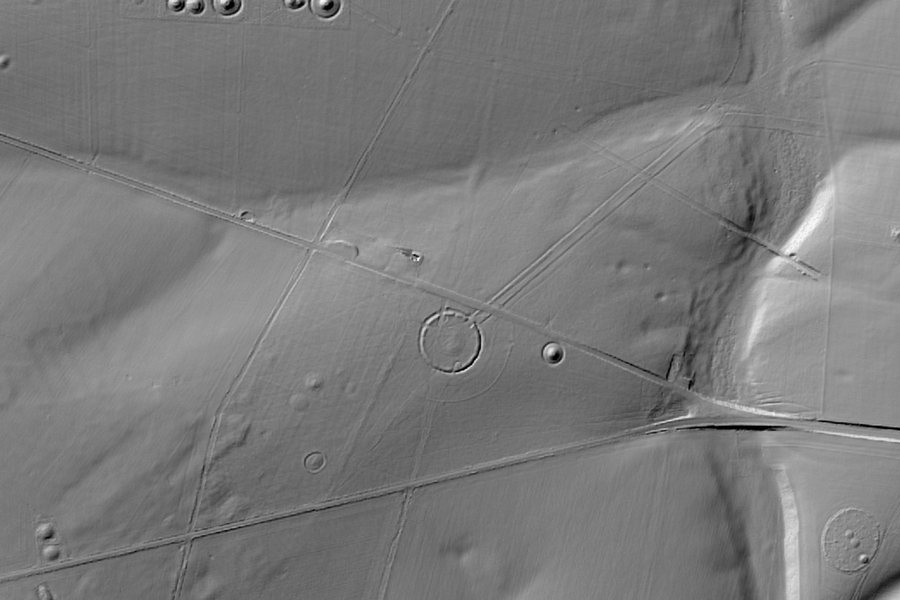
\includegraphics[width=0.86\linewidth]{f_stonehenge.jpg}
\caption*{\textbf{1. Stonehenge and its barrows}, Wiltshire, England. England lidar (Environment Agency, LIDAR Composite DTM).}\end{figure}
Strip away the grass and the stones are the least of it. The bank and ditch round the circle are older than the stones, the Avenue runs off towards the River Avon, and round barrows crowd the ridges on every side. The long, straight Stonehenge Cursus, older again, crosses the downs to the north. \emph{Source: \href{https://en.wikipedia.org/wiki/Stonehenge}{Wikipedia, Stonehenge}.}

\begin{figure}[H]\centering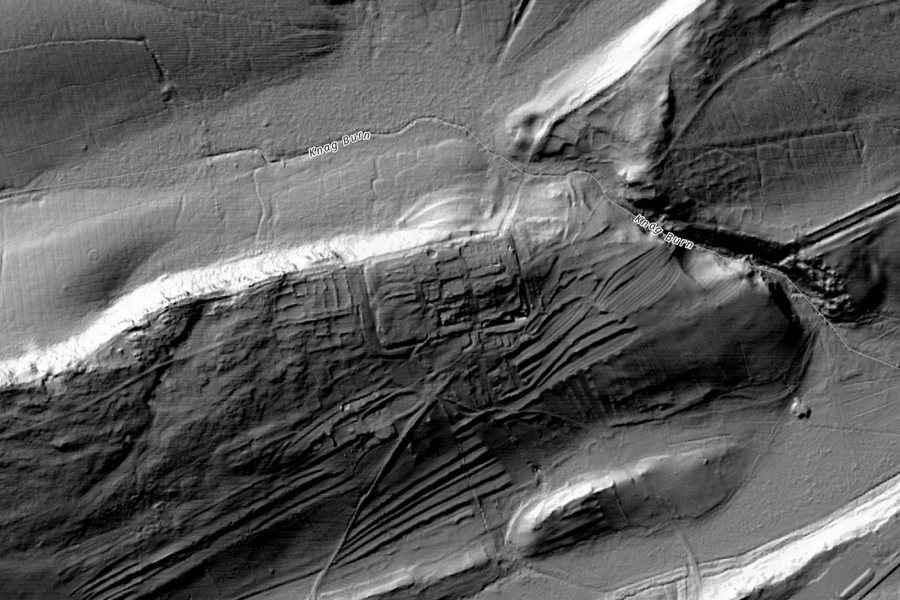
\includegraphics[width=0.86\linewidth]{f_housesteads.jpg}
\caption*{\textbf{2. Hadrian's Wall at Housesteads}, Northumberland, England. England lidar (Environment Agency, LIDAR Composite DTM).}\end{figure}
The Roman fort of Vercovicium sits on the crags of the Whin Sill. South of the Wall the Vallum, a great ditch between two banks dug by the Romans, runs as a double line across the fields. \emph{Source: \href{https://en.wikipedia.org/wiki/Housesteads_Roman_Fort}{Wikipedia, Housesteads Roman Fort}.}

\begin{figure}[H]\centering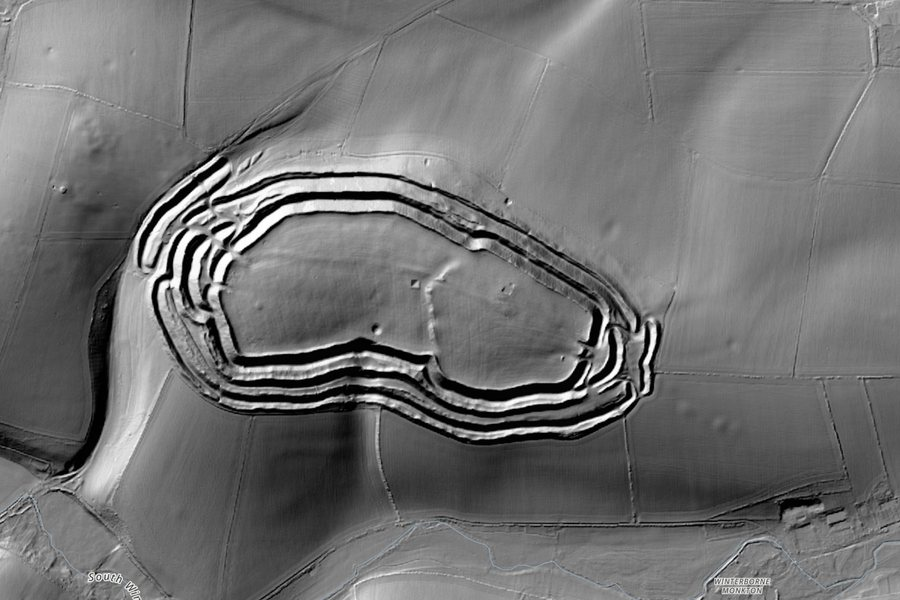
\includegraphics[width=0.86\linewidth]{f_maiden-castle.jpg}
\caption*{\textbf{3. Maiden Castle}, Dorset, England. England lidar (Environment Agency, LIDAR Composite DTM).}\end{figure}
One of the largest Iron Age hillforts in Europe. Lidar shows the rings of ramparts and ditches as clearly as from the air, and the twisting entrances at each end, built so attackers had to walk a maze under the walls. \emph{Source: \href{https://en.wikipedia.org/wiki/Maiden_Castle,_Dorset}{Wikipedia, Maiden Castle, Dorset}.}

\begin{figure}[H]\centering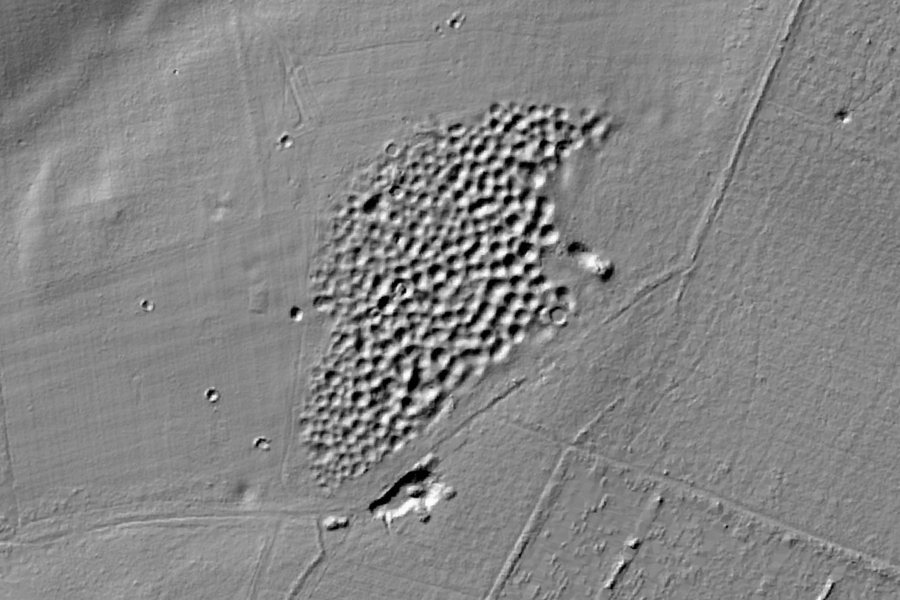
\includegraphics[width=0.86\linewidth]{f_grimes-graves.jpg}
\caption*{\textbf{4. Grime's Graves}, Norfolk, England. England lidar (Environment Agency, LIDAR Composite DTM).}\end{figure}
A field of hollows in the heath, each one the filled-in top of a Neolithic flint mine. More than 400 shafts were dug here about 4,500 years ago to reach the best flint, deep in the chalk. \emph{Source: \href{https://en.wikipedia.org/wiki/Grime's_Graves}{Wikipedia, Grime's Graves}.}

\begin{figure}[H]\centering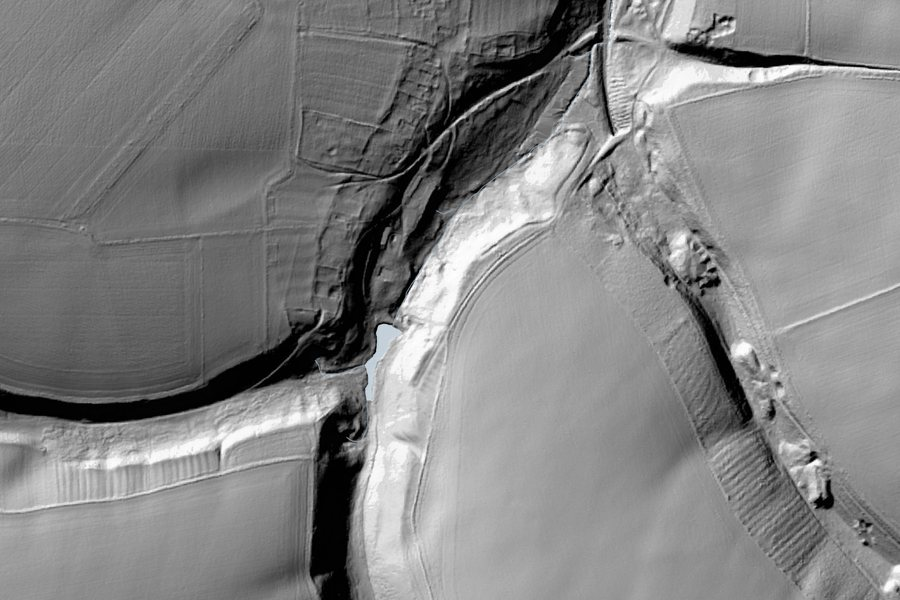
\includegraphics[width=0.86\linewidth]{f_wharram-percy.jpg}
\caption*{\textbf{5. Wharram Percy}, North Yorkshire, England. England lidar (Environment Agency, LIDAR Composite DTM).}\end{figure}
A medieval village that was abandoned around 1500, when its fields were turned over to sheep. The house plots and the strips of ridge and furrow left by medieval ploughs still show in the grass. \emph{Source: \href{https://en.wikipedia.org/wiki/Wharram_Percy}{Wikipedia, Wharram Percy}.}

\begin{figure}[H]\centering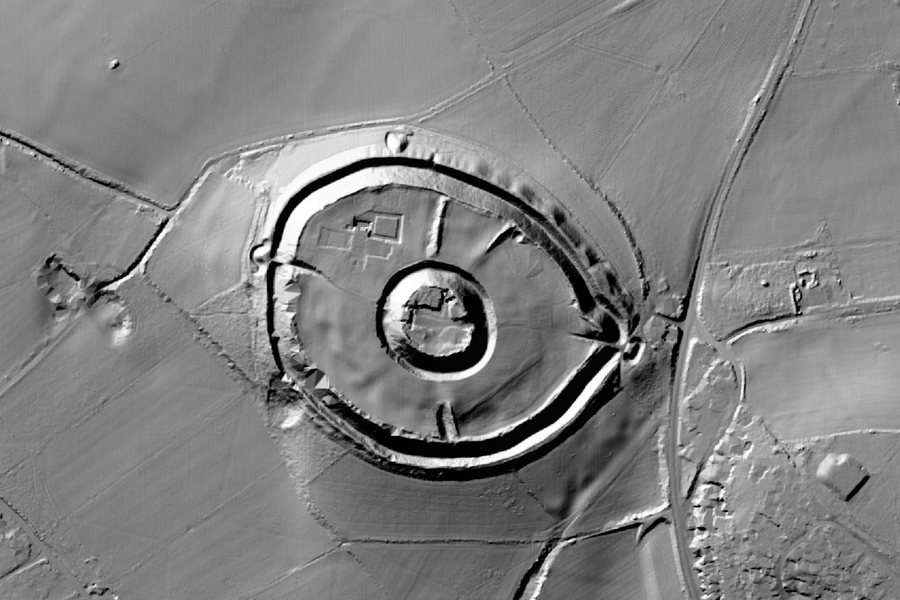
\includegraphics[width=0.86\linewidth]{f_old-sarum.jpg}
\caption*{\textbf{6. Old Sarum}, Wiltshire, England. England lidar (Environment Agency, LIDAR Composite DTM).}\end{figure}
An Iron Age hillfort reused by Romans, Saxons and Normans, who built a castle in the middle and a cathedral beside it. In the 13th century the cathedral moved down to the new Salisbury and the old town slowly emptied, leaving its banks. \emph{Source: \href{https://en.wikipedia.org/wiki/Old_Sarum}{Wikipedia, Old Sarum}.}

\begin{figure}[H]\centering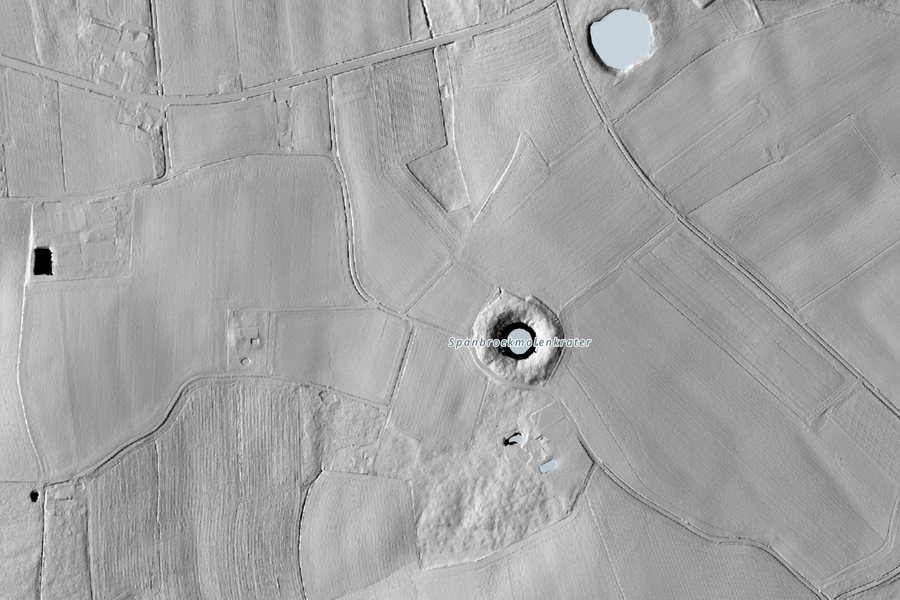
\includegraphics[width=0.86\linewidth]{f_messines.jpg}
\caption*{\textbf{7. The mines of Messines}, West Flanders, Belgium. Flanders lidar (Digitaal Vlaanderen (DHMV II)).}\end{figure}
On 7 June 1917 British tunnellers fired 19 mines under the German lines along the Messines Ridge. Most of the craters are still there, round ponds among the fields; the one at Spanbroekmolen is called the Pool of Peace. Lidar shows its lip of thrown-up earth as a ring. \emph{Source: \href{https://en.wikipedia.org/wiki/Mines_in_the_Battle_of_Messines_(1917)}{Wikipedia, Mines in the Battle of Messines (1917)}.}

\begin{figure}[H]\centering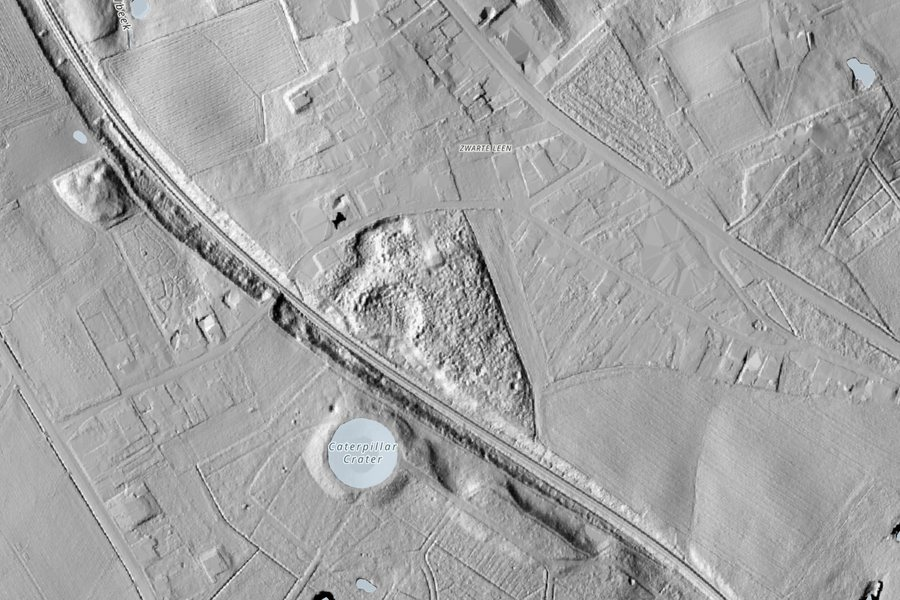
\includegraphics[width=0.86\linewidth]{f_hill-60.jpg}
\caption*{\textbf{8. Hill 60}, Zillebeke, Belgium. Flanders lidar (Digitaal Vlaanderen (DHMV II)).}\end{figure}
A low spoil heap from a railway cutting that both sides fought for from 1914 to 1918, tunnelling beneath it and blowing it apart. Lidar shows a hill turned inside out by craters. \emph{Source: \href{https://en.wikipedia.org/wiki/Hill_60_(Ypres)}{Wikipedia, Hill 60 (Ypres)}.}

\begin{figure}[H]\centering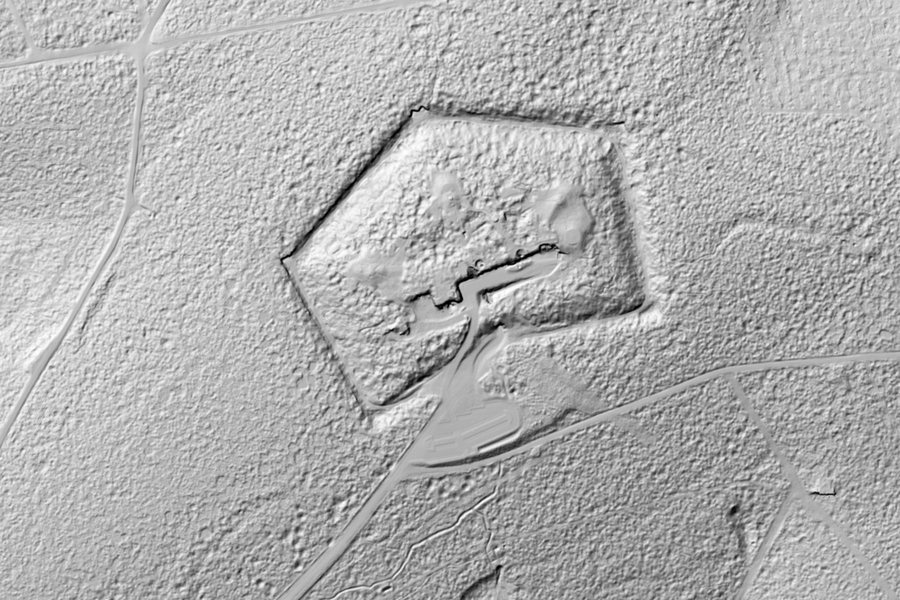
\includegraphics[width=0.86\linewidth]{f_verdun.jpg}
\caption*{\textbf{9. Verdun: Fort Douaumont}, Meuse, France. France lidar (IGN France, LiDAR HD programme).}\end{figure}
The battle of Verdun in 1916 churned this ground with millions of shells. Much of it was too dangerous to farm and was planted with forest. Under the trees, lidar shows every crater, trench and fort as if the guns had only just stopped. \emph{Source: \href{https://en.wikipedia.org/wiki/Fort_Douaumont}{Wikipedia, Fort Douaumont}.}

\begin{figure}[H]\centering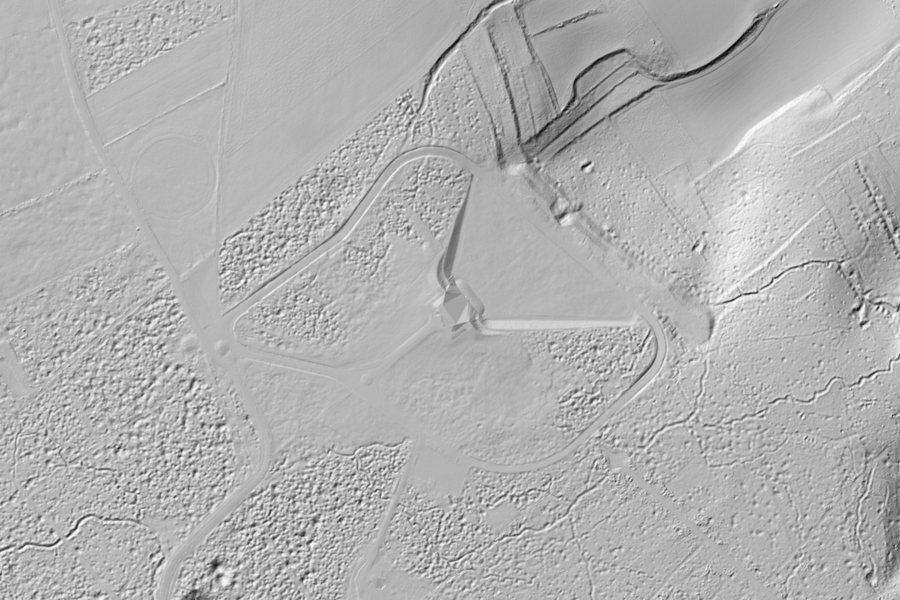
\includegraphics[width=0.86\linewidth]{f_vimy.jpg}
\caption*{\textbf{10. Vimy Ridge}, Pas-de-Calais, France. France lidar (IGN France, LiDAR HD programme).}\end{figure}
In April 1917 the Canadian Corps took this ridge in one of the set-piece attacks of the First World War. The memorial park round the Canadian monument keeps the ground as the battle left it, and under the trees lidar shows shell holes lying lip to lip. \emph{Source: \href{https://en.wikipedia.org/wiki/Canadian_National_Vimy_Memorial}{Wikipedia, Canadian National Vimy Memorial}.}

\begin{figure}[H]\centering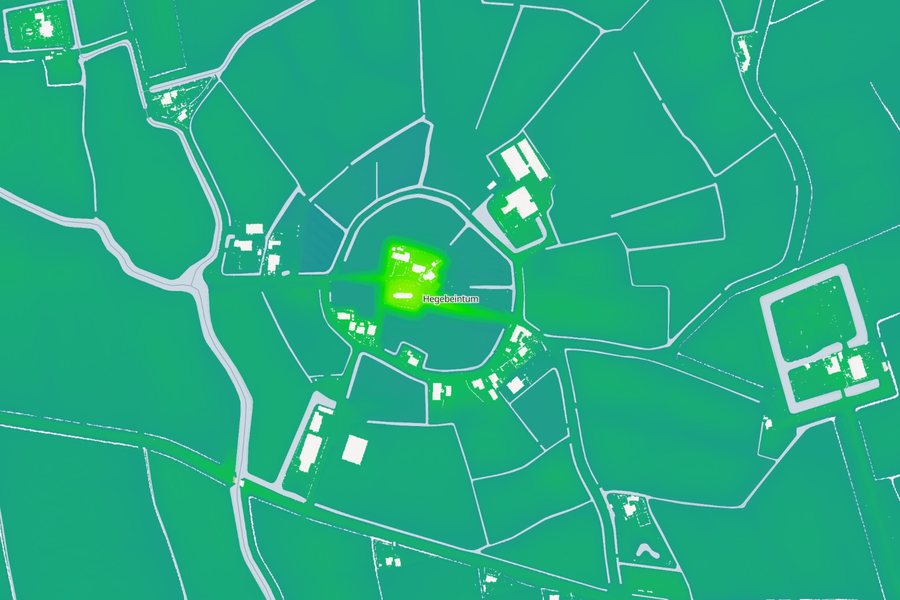
\includegraphics[width=0.86\linewidth]{f_hogebeintum.jpg}
\caption*{\textbf{11. The terp of Hogebeintum}, Friesland, Netherlands. Netherlands lidar (Actueel Hoogtebestand Nederland, via PDOK).}\end{figure}
Before the dykes, people in Friesland lived on mounds they built by hand to keep above the tides. Hogebeintum is the highest left, rising out of land that is otherwise almost perfectly flat. \emph{Source: \href{https://en.wikipedia.org/wiki/Hogebeintum}{Wikipedia, Hogebeintum}.}

\begin{figure}[H]\centering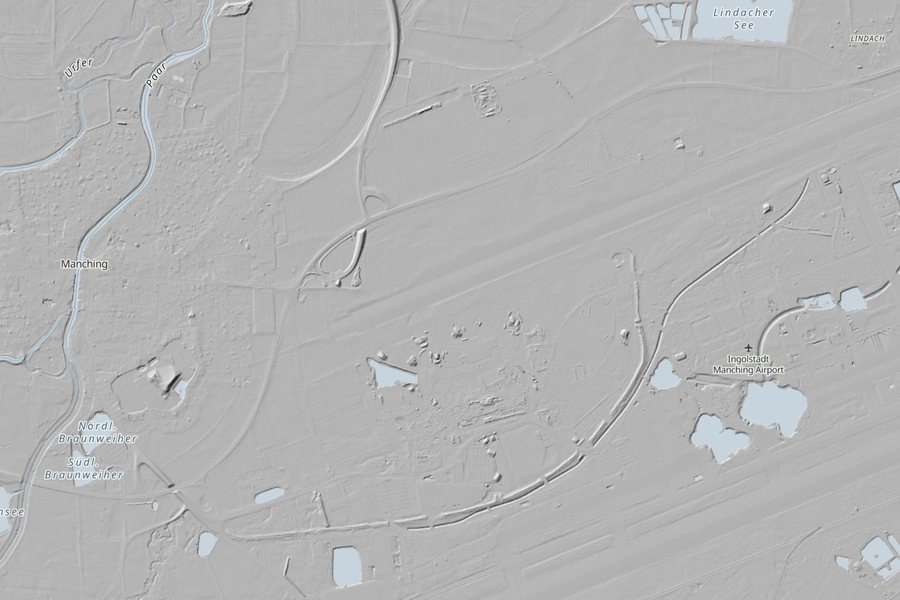
\includegraphics[width=0.86\linewidth]{f_manching.jpg}
\caption*{\textbf{12. The oppidum of Manching}, Bavaria, Germany. Bavaria lidar (Bayerische Vermessungsverwaltung).}\end{figure}
One of the largest Celtic towns north of the Alps. Its wall ran for about 7 km in a near-perfect circle; parts of it still stand, and lidar picks up the rest of the ring across the fields and the airfield. \emph{Source: \href{https://en.wikipedia.org/wiki/Oppidum_of_Manching}{Wikipedia, Oppidum of Manching}.}

\begin{figure}[H]\centering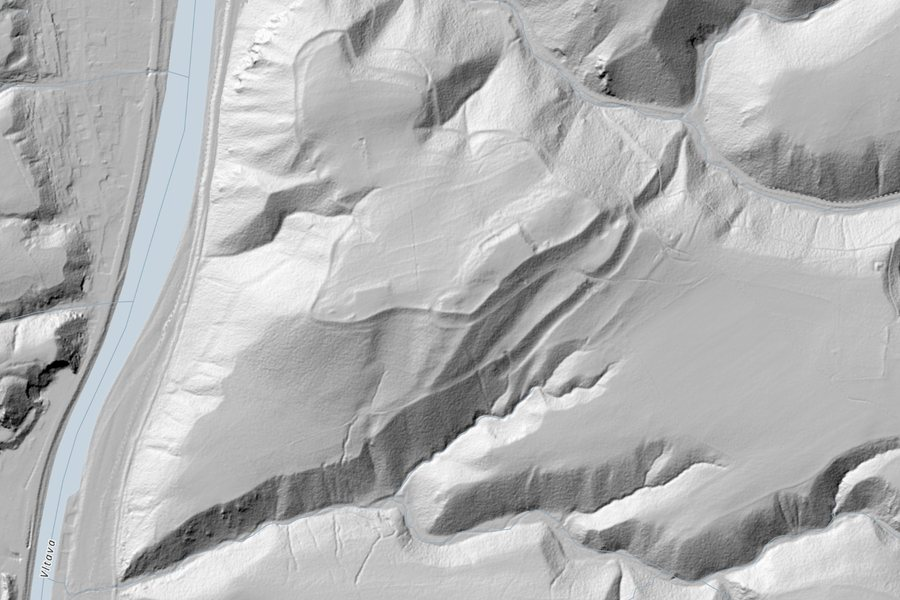
\includegraphics[width=0.86\linewidth]{f_zavist.jpg}
\caption*{\textbf{13. Závist}, Central Bohemia, Czechia. Czechia lidar (ČÚZK, Czech Office for Surveying, Mapping and Cadastre).}\end{figure}
A Celtic hillfort and later oppidum above the Vltava, south of Prague. Its ramparts and terraces lie in woodland, where lidar sees them better than anyone walking through. \emph{Source: \href{https://en.wikipedia.org/wiki/Závist}{Wikipedia, Závist}.}

\begin{figure}[H]\centering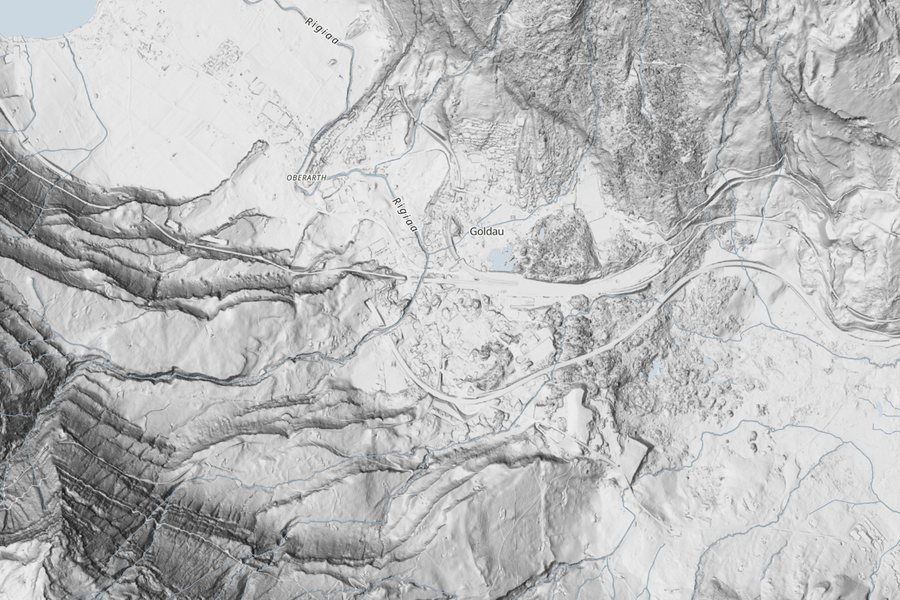
\includegraphics[width=0.86\linewidth]{f_goldau.jpg}
\caption*{\textbf{14. The Goldau landslide}, Schwyz, Switzerland. Switzerland lidar (swisstopo).}\end{figure}
On 2 September 1806 a slab of the Rossberg slid into the valley and buried the village of Goldau, killing 457 people. The scar on the mountain and the rough tongue of rubble below are still plain from above. \emph{Source: \href{https://en.wikipedia.org/wiki/Goldau_landslide}{Wikipedia, Goldau landslide}.}

\begin{figure}[H]\centering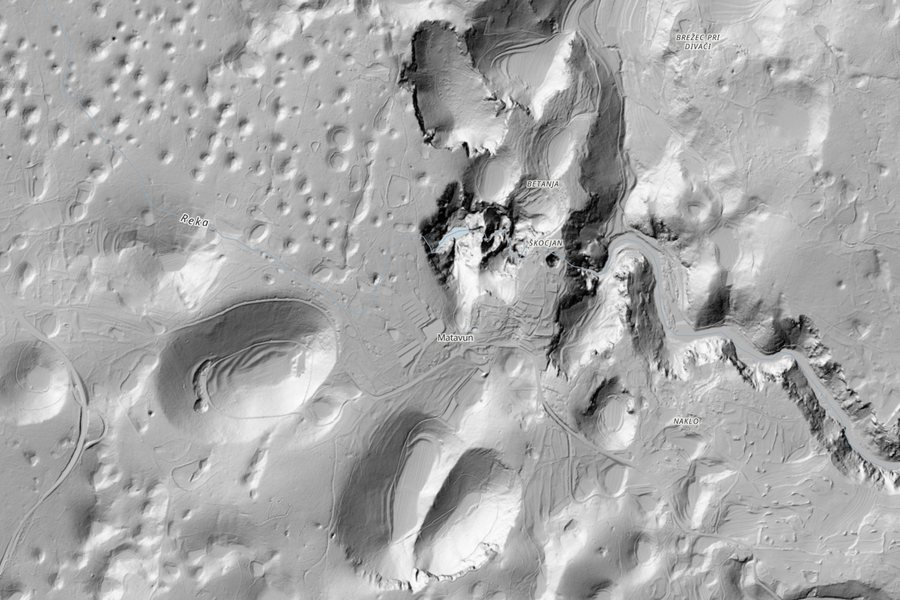
\includegraphics[width=0.86\linewidth]{f_skocjan.jpg}
\caption*{\textbf{15. The karst at Škocjan}, Slovenia. Slovenia lidar (Surveying and Mapping Authority of Slovenia (GURS)).}\end{figure}
The Karst plateau gave the world the word karst. Rain dissolves the limestone from below, so the land is pocked with sinkholes, and at Škocjan two of them are great collapse dolines above one of the largest underground canyons known. \emph{Source: \href{https://en.wikipedia.org/wiki/Škocjan_Caves}{Wikipedia, Škocjan Caves}.}

\begin{figure}[H]\centering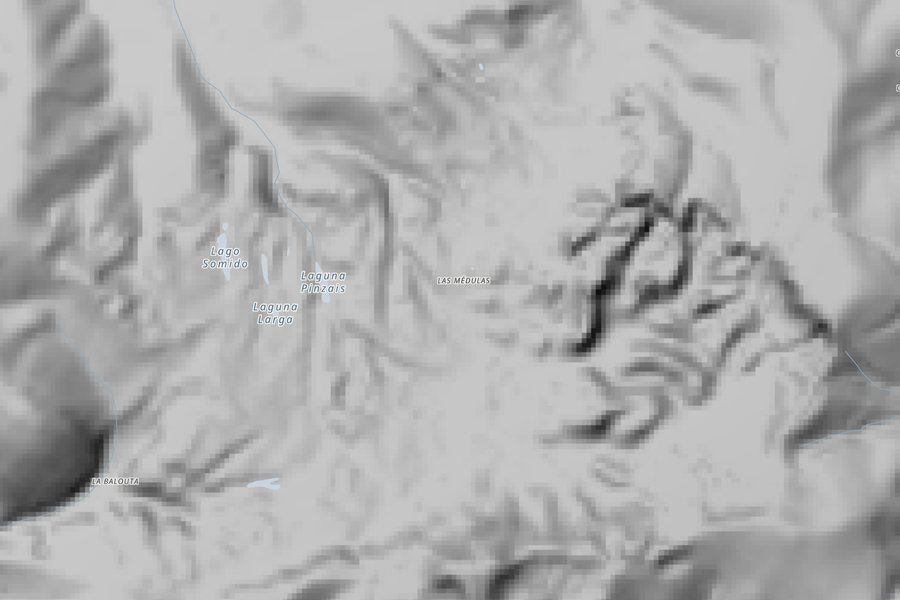
\includegraphics[width=0.86\linewidth]{f_medulas.jpg}
\caption*{\textbf{16. Las Médulas}, León, Spain. Spain lidar (Instituto Geográfico Nacional (IGN), Spain).}\end{figure}
The most important gold mine in the Roman Empire. Roman engineers brought rivers here in channels and used the water to bring down whole hillsides, leaving these red pinnacles and a landscape of tailings and canals. \emph{Source: \href{https://en.wikipedia.org/wiki/Las_Médulas}{Wikipedia, Las Médulas}.}

\begin{figure}[H]\centering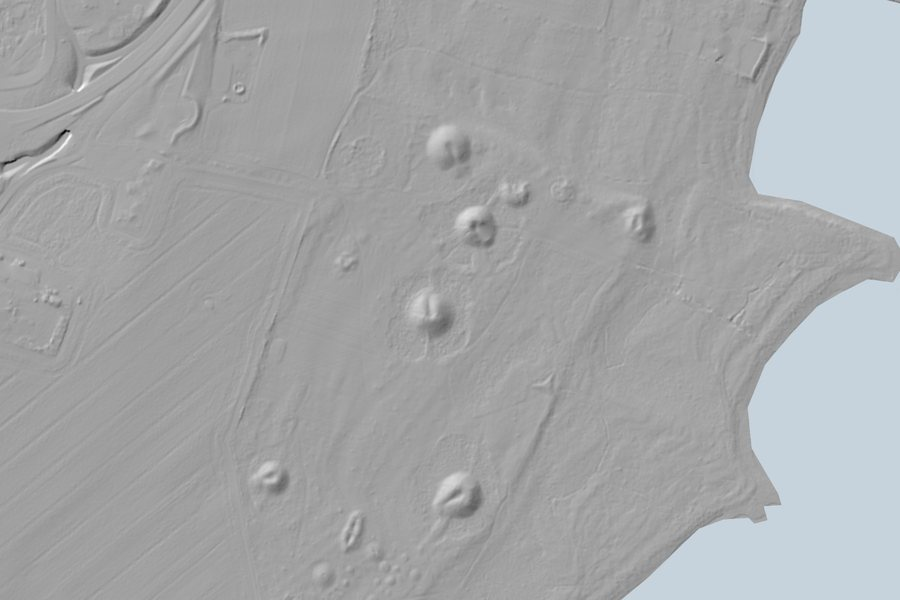
\includegraphics[width=0.86\linewidth]{f_borre.jpg}
\caption*{\textbf{17. The mounds at Borre}, Vestfold, Norway. Norway lidar (Kartverket, Norwegian national detailed elevation model).}\end{figure}
One of the largest groups of grave mounds in Scandinavia, from the Iron Age and the Viking Age. A Viking ship burial was found in one of them in 1852. \emph{Source: \href{https://en.wikipedia.org/wiki/Borre_mound_cemetery}{Wikipedia, Borre mound cemetery}.}

\begin{figure}[H]\centering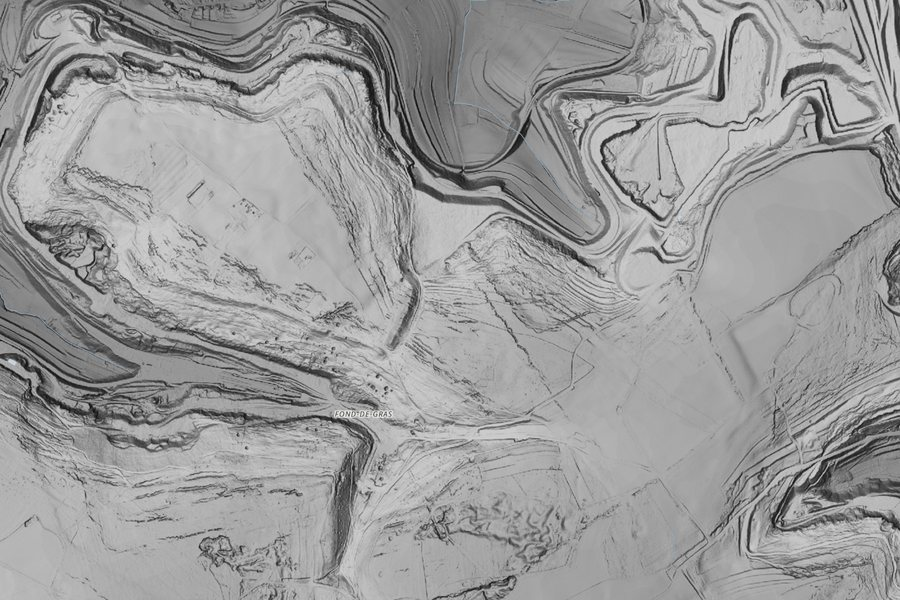
\includegraphics[width=0.86\linewidth]{f_titelberg.jpg}
\caption*{\textbf{18. The Titelberg}, Luxembourg. Luxembourg lidar (Administration du cadastre et de la topographie, Luxembourg).}\end{figure}
An oppidum of the Treveri, a Celtic people, on a plateau above the Chiers. Its earth ramparts still run round the edge of the plateau, and lidar traces them through the woods and fields. \emph{Source: \href{https://en.wikipedia.org/wiki/Titelberg}{Wikipedia, Titelberg}.}

\begin{figure}[H]\centering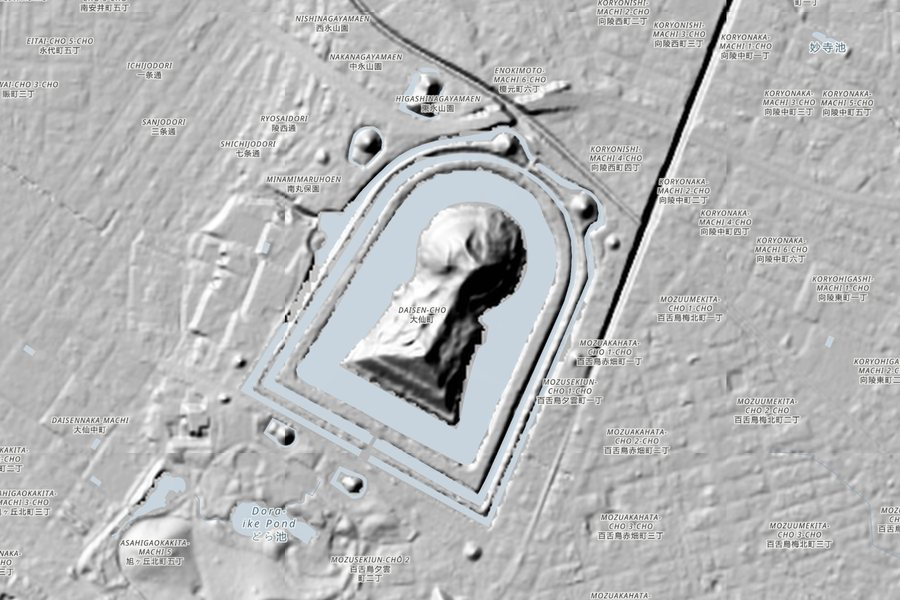
\includegraphics[width=0.86\linewidth]{f_daisen.jpg}
\caption*{\textbf{19. Daisen Kofun}, Sakai, Japan. Japan lidar (Geospatial Information Authority of Japan (GSI)).}\end{figure}
A keyhole-shaped burial mound about 486 m long, the largest in Japan, attributed to the Emperor Nintoku and built in the 5th century. It is closed to the public; its moats and wooded mound are clearest from above. \emph{Source: \href{https://en.wikipedia.org/wiki/Daisen_Kofun}{Wikipedia, Daisen Kofun}.}

\begin{figure}[H]\centering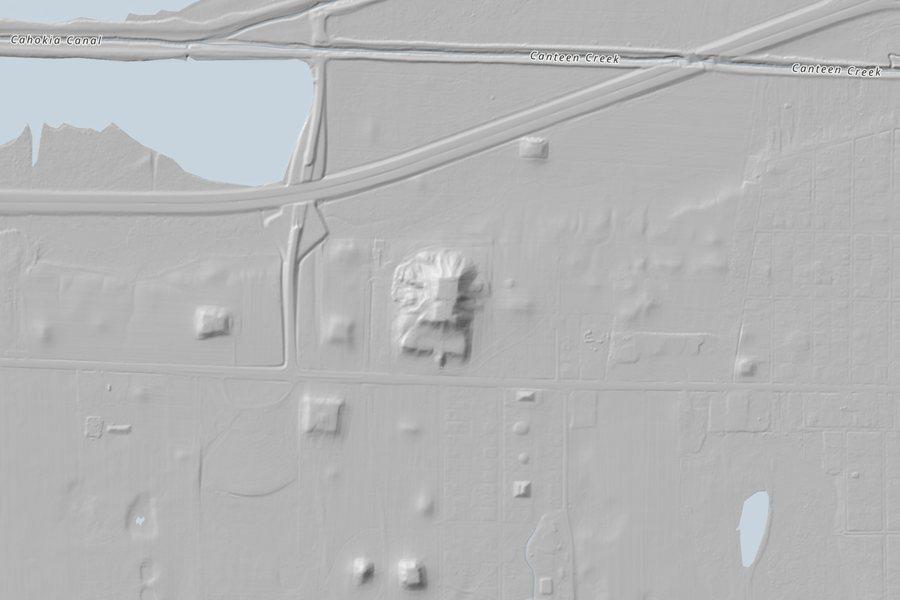
\includegraphics[width=0.86\linewidth]{f_cahokia.jpg}
\caption*{\textbf{20. Cahokia}, Illinois, United States. United States lidar (USGS 3D Elevation Program (3DEP)).}\end{figure}
The largest city north of Mexico before Columbus, at its height around 1100. Monks Mound, made of earth carried by hand in baskets, is the largest prehistoric earthwork in the Americas; smaller mounds stand round it. \emph{Source: \href{https://en.wikipedia.org/wiki/Cahokia}{Wikipedia, Cahokia}.}

\begin{figure}[H]\centering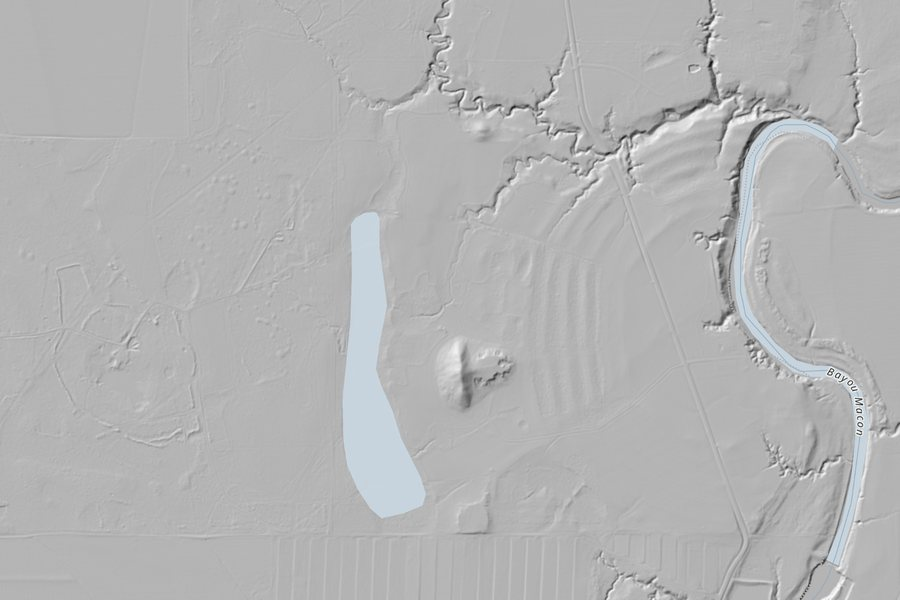
\includegraphics[width=0.86\linewidth]{f_poverty-point.jpg}
\caption*{\textbf{21. Poverty Point}, Louisiana, United States. United States lidar (USGS 3D Elevation Program (3DEP)).}\end{figure}
Six concentric C-shaped ridges and a great bird-shaped mound, built about 3,400 years ago by people who lived by hunting, fishing and gathering. The ridges are low, and easiest to see without the grass. \emph{Source: \href{https://en.wikipedia.org/wiki/Poverty_Point}{Wikipedia, Poverty Point}.}

\begin{figure}[H]\centering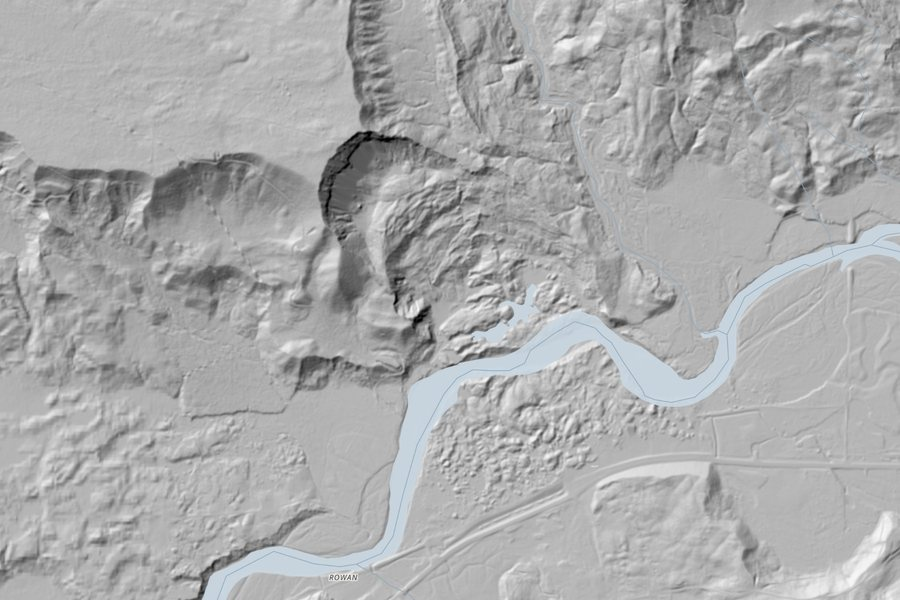
\includegraphics[width=0.86\linewidth]{f_oso.jpg}
\caption*{\textbf{22. The Oso landslide}, Washington, United States. United States lidar (USGS 3D Elevation Program (3DEP)).}\end{figure}
On 22 March 2014 a hillside above the North Fork Stillaguamish River gave way, burying a neighbourhood and killing 43 people. Lidar flown before the slide showed older landslides here, but few had looked. \emph{Source: \href{https://en.wikipedia.org/wiki/2014_Oso_mudslide}{Wikipedia, 2014 Oso mudslide}.}

\begin{figure}[H]\centering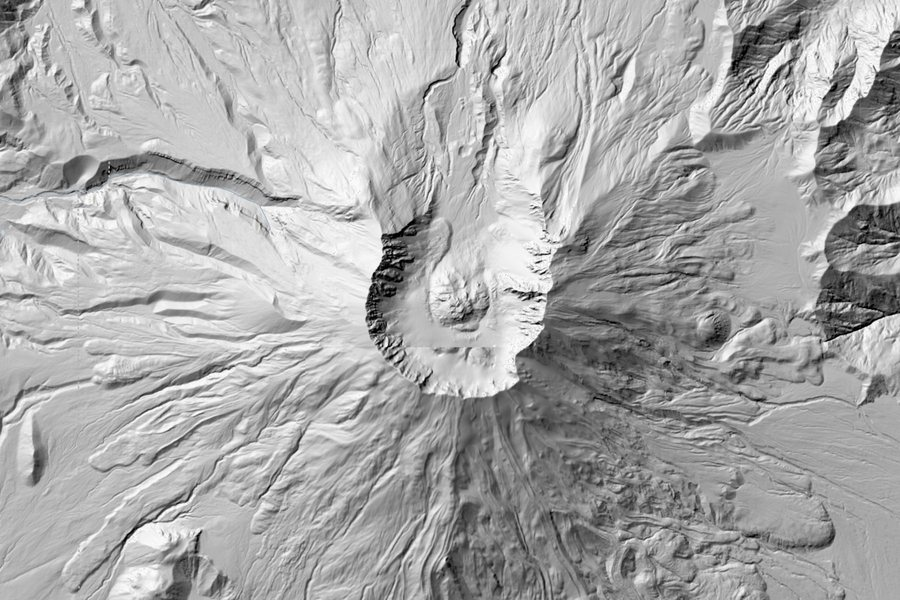
\includegraphics[width=0.86\linewidth]{f_st-helens.jpg}
\caption*{\textbf{23. Mount St Helens}, Washington, United States. United States lidar (USGS 3D Elevation Program (3DEP)).}\end{figure}
On 18 May 1980 the north face of the volcano collapsed in the largest landslide on record and the blast flattened forest for miles. The horseshoe crater, the new dome inside it and the debris below are clearer in lidar than in any photograph. \emph{Source: \href{https://en.wikipedia.org/wiki/Mount_St._Helens}{Wikipedia, Mount St. Helens}.}

\section*{Data and code}
Map, layer list, coverage outlines, gallery and this paper: \url{https://github.com/Tristan-Hotham/lidar-world} and DOI \href{https://doi.org/10.5281/zenodo.23866756}{10.5281/zenodo.23866756}. Code MIT; text, gallery notes and figures CC BY 4.0. The shaded relief in the figures belongs to the publishers in Table~1, used under their licences; world shaded relief by Esri. The author used an AI system to help draft code and text, and checked every factual claim against the sources given.
\end{document}
